\documentclass[12pt,a4paper]{report}

\usepackage[margin=1in]{geometry}
\usepackage[T1]{fontenc}
\usepackage{lmodern}
\usepackage{microtype}
\usepackage{graphicx}
\usepackage{xcolor}
\usepackage{booktabs}
\usepackage{array}
\usepackage{enumitem}
\usepackage{listings}
\usepackage{tikz}
\usepackage[hidelinks]{hyperref}
\usetikzlibrary{positioning,arrows.meta}

\setlength{\parskip}{0.45em}
\setlength{\parindent}{0pt}
\renewcommand{\arraystretch}{1.2}
\setlist[itemize]{leftmargin=1.5em}

\definecolor{codebg}{RGB}{246,248,250}
\definecolor{codeborder}{RGB}{210,215,220}
\definecolor{sqlblue}{RGB}{30,75,150}
\definecolor{sqlgreen}{RGB}{30,120,70}

\lstdefinestyle{sqlstyle}{
    language=SQL,
    basicstyle=\ttfamily\small,
    keywordstyle=\color{sqlblue}\bfseries,
    commentstyle=\color{sqlgreen},
    stringstyle=\color{red!65!black},
    backgroundcolor=\color{codebg},
    frame=single,
    rulecolor=\color{codeborder},
    breaklines=true,
    showstringspaces=false,
    columns=fullflexible,
    keepspaces=true
}

\newcommand{\studentname}{Shreyas Vishwakarma}
\newcommand{\studentroll}{Your Roll Number}
\newcommand{\coursename}{BCA / Your Course}
\newcommand{\departmentname}{Department of Computer Science}
\newcommand{\collegename}{Deep}
\newcommand{\guidename}{Project Guide Name}
\newcommand{\submissiondate}{October 2026}

\newcommand{\screenshotplaceholder}[2]{%
    \IfFileExists{screenshots/#1}{%
        \includegraphics[width=0.94\textwidth,height=0.52\textheight,keepaspectratio]{screenshots/#1}%
    }{%
        \fbox{\parbox[c][4.2cm][c]{0.88\textwidth}{%
            \centering Add your MySQL Workbench screenshot here\\[0.5em]
            \texttt{screenshots/#1}\\[0.5em]
            \small #2%
        }}%
    }%
}

\begin{document}

\begin{titlepage}
    \centering
    \vspace*{1.5cm}
    {\Large\bfseries \collegename\par}
    \vspace{0.4cm}
    {\large \departmentname\par}
    \vspace{2.0cm}
    {\Huge\bfseries Student Attendance\\[0.25em] Management System\par}
    \vspace{1.0cm}
    {\Large Database Mini Project Report\par}
    \vspace{1.7cm}
    {\large Submitted in partial fulfillment of the requirements for\\
    \coursename\par}
    \vspace{1.2cm}
    \begin{tabular}{>{\bfseries}rl}
        Submitted by: & \studentname \\
        Roll number: & \studentroll \\
        Project guide: & \guidename \\
        Submission date: & \submissiondate
    \end{tabular}
    \vfill
    {\large \collegename\par}
\end{titlepage}

\pagenumbering{roman}

\chapter*{Certificate}
\addcontentsline{toc}{chapter}{Certificate}
This is to certify that the mini project entitled \textbf{Student Attendance Management System} is submitted by \textbf{\studentname} (\studentroll) as part of the academic work for \coursename\ in \submissiondate.

\vspace{2cm}
\begin{tabular*}{\textwidth}{@{\extracolsep{\fill}}ll}
    \rule{5cm}{0.4pt} & \rule{5cm}{0.4pt} \\
    Project Guide & Head of Department
\end{tabular*}

\chapter*{Acknowledgement}
\addcontentsline{toc}{chapter}{Acknowledgement}
I express my sincere gratitude to my project guide, faculty members, and institution for their guidance and support during this mini project. I also thank everyone who provided feedback that helped me complete and document the database work.

\chapter*{Abstract}
\addcontentsline{toc}{chapter}{Abstract}
The Student Attendance Management System is a MySQL database mini project for organizing student, teacher, subject, and attendance information. It uses relational tables, primary and foreign keys, uniqueness rules, and SQL queries to retrieve attendance details and generate summaries. The demonstration queries calculate attendance percentages and daily or subject-wise counts. For this project, a late mark is counted as attended when calculating the percentage. The database can be operated in MySQL Workbench; this submission is a database implementation and does not claim to include a separate graphical application.

\tableofcontents
\clearpage
\pagenumbering{arabic}

\chapter{Introduction}
Attendance records help institutions monitor student participation and identify attendance issues. Paper-based record keeping can be difficult to update and summarize. This project demonstrates how a relational database can keep attendance records organized and support repeatable reports.

\section{Problem Statement}
Manual attendance records may be inconsistent, difficult to search, and time-consuming to summarize by student, subject, or date. A structured database is needed to link attendance entries with their students, subjects, and teachers and to retrieve summary information through SQL.

\section{Objectives}
\begin{itemize}
    \item Store student, teacher, and subject details in structured tables.
    \item Record a student's attendance status for a subject on a date.
    \item Prevent duplicate attendance entries for a student, subject, and date.
    \item Retrieve attendance history and calculate attendance percentages.
    \item Produce subject-wise and date-wise attendance summaries.
\end{itemize}

\section{Scope}
The scope of this mini project is the MySQL schema, sample records, and demonstration SQL queries. Login, role-based permissions, a graphical user interface, notifications, and integration with a college information system are outside the current implementation.

\chapter{Requirements and Design}
\section{Software and Hardware Requirements}
\begin{itemize}
    \item MySQL Server 8.0 or newer
    \item MySQL Workbench
    \item A computer capable of running MySQL Server and Workbench
\end{itemize}

\section{System Modules}
\begin{itemize}
    \item Student record management
    \item Teacher record management
    \item Subject record management
    \item Attendance recording and correction
    \item Attendance listing and report queries
\end{itemize}

\section{Entity Relationship Model}
The \texttt{attendance} table is the transaction table. Each attendance row refers to exactly one student, subject, and teacher. Each of those records can be associated with multiple attendance rows.

\begin{figure}[htbp]
\centering
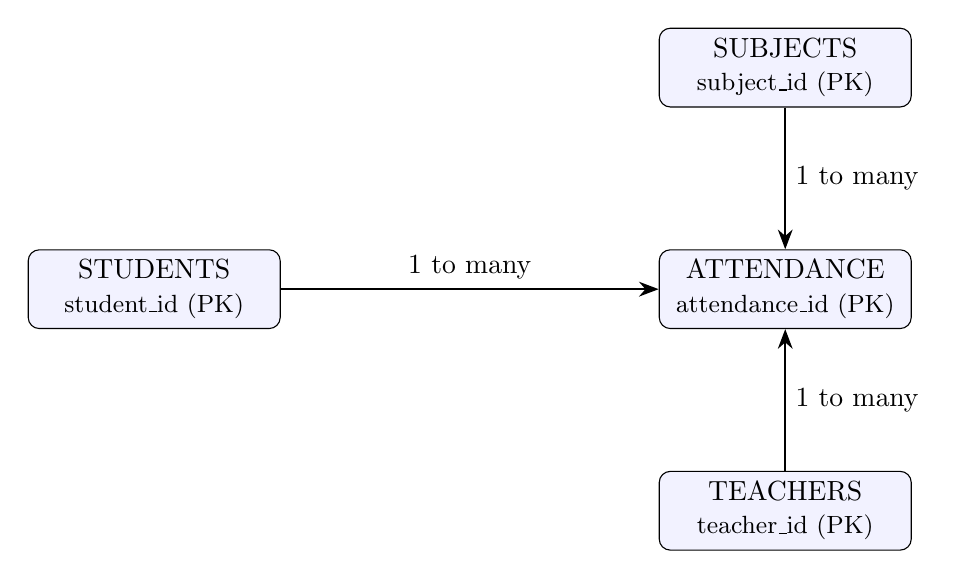
\begin{tikzpicture}[
    entity/.style={draw, rounded corners, align=center, minimum width=3.2cm, minimum height=1cm, fill=blue!5},
    relation/.style={-{Stealth[length=2.5mm]}, thick}
]
    \node[entity] (students) {STUDENTS\\\small student\_id (PK)};
    \node[entity, right=4.8cm of students] (attendance) {ATTENDANCE\\\small attendance\_id (PK)};
    \node[entity, above=1.8cm of attendance] (subjects) {SUBJECTS\\\small subject\_id (PK)};
    \node[entity, below=1.8cm of attendance] (teachers) {TEACHERS\\\small teacher\_id (PK)};
    \draw[relation] (students) -- node[above,sloped]{1 to many} (attendance);
    \draw[relation] (subjects) -- node[right]{1 to many} (attendance);
    \draw[relation] (teachers) -- node[right]{1 to many} (attendance);
\end{tikzpicture}
\caption{Conceptual entity relationship diagram}
\end{figure}

\section{Relational Tables}
\begin{table}[htbp]
\centering
\begin{tabular}{p{3cm}p{10cm}}
\toprule
\textbf{Table} & \textbf{Purpose and key fields} \\
\midrule
\texttt{students} & Student profile; primary key \texttt{student\_id}, unique \texttt{roll\_no}. \\
\texttt{teachers} & Teacher profile; primary key \texttt{teacher\_id}. \\
\texttt{subjects} & Subject details; primary key \texttt{subject\_id}, unique \texttt{subject\_code}. \\
\texttt{attendance} & Attendance events; foreign keys reference student, subject, and teacher. A unique key prevents duplicate student-subject-date entries. \\
\bottomrule
\end{tabular}
\caption{Database tables}
\end{table}

\section{Attendance Status and Percentage Rule}
The status code \texttt{P} means Present, \texttt{A} means Absent, and \texttt{L} means Late. The example percentage formula counts both Present and Late as attended:
\[
\text{Attendance percentage} =
\frac{\text{Present sessions}+\text{Late sessions}}{\text{All marked sessions}}
\times 100.
\]
The institution's attendance policy should be followed if it treats late arrivals differently.

\chapter{Database Implementation}
The full setup script is provided in \texttt{student\_attendance.sql}. It creates the database, tables, constraints, and sample data. Run that file in MySQL Workbench as described in \texttt{MYSQL\_WORKBENCH\_GUIDE.md}.

\section{Table Creation}
\lstinputlisting[style=sqlstyle, firstline=1, lastline=63, caption={Database and relational table definitions}]{student_attendance.sql}

\section{Sample Attendance Query}
\begin{lstlisting}[style=sqlstyle, caption={Joining attendance to student, subject, and teacher details}]
SELECT
    a.attendance_date,
    s.roll_no,
    s.student_name,
    sub.subject_name,
    t.teacher_name,
    a.status
FROM attendance AS a
JOIN students AS s ON s.student_id = a.student_id
JOIN subjects AS sub ON sub.subject_id = a.subject_id
JOIN teachers AS t ON t.teacher_id = a.teacher_id
ORDER BY a.attendance_date, sub.subject_name, s.roll_no;
\end{lstlisting}

\section{Attendance Percentage Query}
\begin{lstlisting}[style=sqlstyle, caption={Percentage per student and subject; late marks count as attended}]
SELECT
    s.roll_no,
    s.student_name,
    sub.subject_name,
    COUNT(a.attendance_id) AS sessions_held,
    SUM(CASE WHEN a.status IN ('P', 'L') THEN 1 ELSE 0 END)
        AS sessions_attended,
    ROUND(
        100.0 * SUM(CASE WHEN a.status IN ('P', 'L') THEN 1 ELSE 0 END)
        / NULLIF(COUNT(a.attendance_id), 0),
        2
    ) AS attendance_percentage
FROM students AS s
CROSS JOIN subjects AS sub
LEFT JOIN attendance AS a
    ON a.student_id = s.student_id
   AND a.subject_id = sub.subject_id
GROUP BY s.student_id, s.roll_no, s.student_name,
         sub.subject_id, sub.subject_name
ORDER BY s.roll_no, sub.subject_name;
\end{lstlisting}

\section{Sample Data Summary}
\begin{table}[htbp]
\centering
\begin{tabular}{lrrr}
\toprule
\textbf{Subject} & \textbf{Present} & \textbf{Absent} & \textbf{Late} \\
\midrule
Database Management Systems & 3 & 1 & 1 \\
Java Programming & 4 & 1 & 0 \\
Operating Systems & 3 & 1 & 1 \\
\bottomrule
\end{tabular}
\caption{Expected subject-wise counts for the supplied sample data}
\end{table}

\chapter{Execution and Results}
\section{Execution Procedure}
\begin{enumerate}
    \item Open MySQL Workbench and connect to the local MySQL Server.
    \item Open \texttt{student\_attendance.sql} and execute the full script.
    \item Refresh the Schemas panel and verify the database and four tables.
    \item Run each demonstration \texttt{SELECT} query separately.
    \item Capture the query and Result Grid for the evidence pages below.
\end{enumerate}

\section{Database and Tables}
\begin{figure}[htbp]
\centering
\screenshotplaceholder{01-database-and-tables.png}{Workbench schema tree showing student\_attendance\_db and its tables}
\caption{Database and tables in MySQL Workbench}
\end{figure}

\section{Student Listing}
\begin{figure}[htbp]
\centering
\screenshotplaceholder{02-student-list.png}{Student-list SQL query and the result grid}
\caption{Student records}
\end{figure}

\section{Attendance Details}
\begin{figure}[htbp]
\centering
\screenshotplaceholder{03-attendance-details.png}{Joined attendance query and the result grid}
\caption{Attendance details with related names}
\end{figure}

\section{Attendance Percentage}
\begin{figure}[htbp]
\centering
\screenshotplaceholder{04-attendance-percentage.png}{Percentage query and the result grid}
\caption{Attendance percentage by student and subject}
\end{figure}

\section{Attendance Summaries}
\begin{figure}[htbp]
\centering
\screenshotplaceholder{05-subject-summary.png}{Subject-wise Present, Absent, and Late counts}
\caption{Subject-wise attendance summary}
\end{figure}
\begin{figure}[htbp]
\centering
\screenshotplaceholder{06-daily-summary.png}{Date-wise Present, Absent, and Late counts}
\caption{Daily attendance summary}
\end{figure}

\chapter{Conclusion and Future Scope}
This project demonstrates how MySQL can organize attendance records using related tables, primary keys, foreign keys, and uniqueness constraints. The supplied queries retrieve attendance history and calculate student, subject, and daily summaries. A future version could add a user interface, authentication, multiple class sessions per day, access permissions, and exportable reports.

\chapter*{References}
\addcontentsline{toc}{chapter}{References}
\begin{enumerate}
    \item MySQL 8.0 Reference Manual, \url{https://dev.mysql.com/doc/refman/8.0/en/}
    \item MySQL Workbench Manual, \url{https://dev.mysql.com/doc/workbench/en/}
\end{enumerate}

\end{document}
